\chapter{REPORTE FOTOGRÁFICO.} %(((

En los activos 1, 2, 3, 4, 5, 6, 7, 8, 9, 10, 11, 23, 24, 25, 26, 27, 28, 29, no se obtuvo reporte fotográfico.

\begin{figure}[hbtp!]
	\centering
	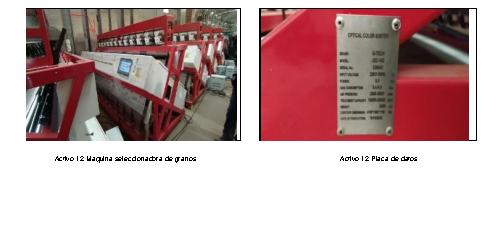
\includegraphics[width=  \linewidth, page = 1]{../0.imagenes/CAP_12/cap_12}
\end{figure}
\newpage

\begin{figure}[hbtp!]
	\centering
	\includegraphics[width=  \linewidth, page = 2]{../0.imagenes/CAP_12/cap_12}
\end{figure}
\newpage

\begin{figure}[hbtp!]
	\centering
	\includegraphics[width=  \linewidth, page = 3]{../0.imagenes/CAP_12/cap_12}
\end{figure}
\newpage

\begin{figure}[hbtp!]
	\centering
	\includegraphics[width=  \linewidth, page = 4]{../0.imagenes/CAP_12/cap_12}
\end{figure}
\newpage

\begin{figure}[hbtp!]
	\centering
	\includegraphics[width=  \linewidth, page = 5]{../0.imagenes/CAP_12/cap_12}
\end{figure}
\newpage

\begin{figure}[hbtp!]
	\centering
	\includegraphics[width=  \linewidth, page = 6]{../0.imagenes/CAP_12/cap_12}
\end{figure}
\newpage

\begin{figure}[hbtp!]
	\centering
	\includegraphics[width=  \linewidth, page = 7]{../0.imagenes/CAP_12/cap_12}
\end{figure}
\newpage

\begin{figure}[hbtp!]
	\centering
	\includegraphics[width=  \linewidth, page = 8]{../0.imagenes/CAP_12/cap_12}
\end{figure}
\newpage

\begin{figure}[hbtp!]
	\centering
	\includegraphics[width=  \linewidth, page = 9]{../0.imagenes/CAP_12/cap_12}
\end{figure}
\newpage

\begin{figure}[hbtp!]
	\centering
	\includegraphics[width=  \linewidth, page = 10]{../0.imagenes/CAP_12/cap_12}
\end{figure}
\newpage

\begin{figure}[hbtp!]
	\centering
	\includegraphics[width=  \linewidth, page = 11]{../0.imagenes/CAP_12/cap_12}
\end{figure}
\newpage

\begin{figure}[hbtp!]
	\centering
	\includegraphics[width=  \linewidth, page = 12]{../0.imagenes/CAP_12/cap_12}
\end{figure}
\newpage

\begin{figure}[hbtp!]
	\centering
	\includegraphics[width=  \linewidth, page = 15]{../0.imagenes/CAP_12/cap_12}
\end{figure}
\newpage

\begin{figure}[hbtp!]
	\centering
	\includegraphics[width=  \linewidth, page = 16]{../0.imagenes/CAP_12/cap_12}
\end{figure}
\newpage

\begin{figure}[hbtp!]
	\centering
	\includegraphics[width=  \linewidth, page = 17]{../0.imagenes/CAP_12/cap_12}
\end{figure}
\newpage

\begin{figure}[hbtp!]
	\centering
	\includegraphics[width=  \linewidth, page = 18]{../0.imagenes/CAP_12/cap_12}
\end{figure}
\newpage

\begin{figure}[hbtp!]
	\centering
	\includegraphics[width=  \linewidth, page = 19]{../0.imagenes/CAP_12/cap_12}
\end{figure}
\newpage

\begin{figure}[hbtp!]
	\centering
	\includegraphics[width=  \linewidth, page = 20]{../0.imagenes/CAP_12/cap_12}
\end{figure}
\newpage

\begin{figure}[hbtp!]
	\centering
	\includegraphics[width=  \linewidth, page = 21]{../0.imagenes/CAP_12/cap_12}
\end{figure}
\newpage

\begin{figure}[hbtp!]
	\centering
	\includegraphics[width=  \linewidth, page = 22]{../0.imagenes/CAP_12/cap_12}
\end{figure}
\newpage

\begin{figure}[hbtp!]
	\centering
	\includegraphics[width=  \linewidth, page = 23]{../0.imagenes/CAP_12/cap_12}
\end{figure}
\newpage

\begin{figure}[hbtp!]
	\centering
	\includegraphics[width=  \linewidth, page = 24]{../0.imagenes/CAP_12/cap_12}
\end{figure}
\newpage

\begin{figure}[hbtp!]
	\centering
	\includegraphics[width=  \linewidth, page = 25]{../0.imagenes/CAP_12/cap_12}
\end{figure}
\newpage

\begin{figure}[hbtp!]
	\centering
	\includegraphics[width=  \linewidth, page = 26]{../0.imagenes/CAP_12/cap_12}
\end{figure}
\newpage

\begin{figure}[hbtp!]
	\centering
	\includegraphics[width=  \linewidth, page = 27]{../0.imagenes/CAP_12/cap_12}
\end{figure}
\newpage

\begin{figure}[hbtp!]
	\centering
	\includegraphics[width=  \linewidth, page = 28]{../0.imagenes/CAP_12/cap_12}
\end{figure}
\newpage

\begin{figure}[hbtp!]
	\centering
	\includegraphics[width=  \linewidth, page = 29]{../0.imagenes/CAP_12/cap_12}
\end{figure}
\newpage

\begin{figure}[hbtp!]
	\centering
	\includegraphics[width=  \linewidth, page = 30]{../0.imagenes/CAP_12/cap_12}
\end{figure}
\newpage

\begin{figure}[hbtp!]
	\centering
	\includegraphics[width=  \linewidth, page = 31]{../0.imagenes/CAP_12/cap_12}
\end{figure}
\newpage

% )))
